\section{From acceptance to identification}
\label{sec:identification}

Apply Proposition~\ref{prop:computation} to the fixed machine \(M\) and input
\(w\).  We turn its circuit description into comparison schemas, then use the
graph construction of the preceding sections.  The additional comparisons
serve two purposes: an accepting test will force singleton values at every
gate type and at an additional broadcast type, at all addresses, and coordinate
self-connections will make those values row-sum functions.  Both properties
are needed to identify the graph among all its equivalent mates.

\subsection{Real types and buffered connections}

Give each scalar gate type dimension one, with its scalar coordinate as both
input and output form.  Give each AND type dimension two: the input forms are
the coordinate projections and the output form is their sum.  Introduce a
further scalar type \(A\), called the broadcast type.  The gate types and
\(A\) will be called the \emph{primary types}.  Also introduce a scalar dummy
type.  For each seed request, add a comparison from the specified scalar
type to the dummy on that request's product domain, with identity address
transmission, comparing the scalar form at the source with the zero form at
the dummy.  The dummy has no other use.

Regard the circuit connections as directed connections from a source output
form to a destination input form.  Add the following directed connection
schemas:
\begin{enumerate}
\item From each tested scalar type to \(A\), on its test domain and with
identity address transmission.
\item For each address coordinate \(i\), from \(A\) to \(A\) on the full
product, flipping coordinate \(i\) and leaving the others unchanged.
\item From \(A\) to every coordinate form of every gate type, on the full
product with identity address transmission.
\item From every coordinate form of every primary type to itself, on the full
product with identity address transmission.  For the coordinate of \(A\),
include two distinct copies of this self-connection.
\end{enumerate}
These added connections describe constraints; they are not included when
evaluating the acyclic circuit from Section~\ref{sec:computation}.

One-way propagation is a central feature of Grohe's monotone-circuit
reductions for finite-variable equivalence~\cite{Grohe1999} and of the
later identification construction of Lichter, Ra\ss mann, and Schweitzer
\cite[Section~5]{LRS2025}. Here private two-coordinate scalar-image
buffers implement the directional effect. Their exact properties,
including the shifted comparisons needed for arbitrary mates, are
proved below rather than imported from those graph switches.

Implement each directed connection schema \(l\), original or added, using a
private real type \(B_l\) of dimension two.  Suppose \(l\) goes from a form
\(o\) on a primary type \(P\) to a form \(s\) on a primary type \(R\), with
source domain \(D_l\) and address map \(\sigma_l\).  The two coordinate
forms of \(B_l\) are denoted by \(z_1,z_2\), and its addresses use the source
coordinate system.  Add precisely three comparison schemas:
\begin{equation}
\begin{array}{c|c|c|c}
 \text{schema}&\text{source form}&\text{destination form}
       &\text{address map on }D_l\\ \hline
 l1&o\text{ on }P&z_1\text{ on }B_l&\mathrm{id}\\
 l2&o\text{ on }P&z_2\text{ on }B_l&\mathrm{id}\\
 l3&z_1+z_2\text{ on }B_l&s\text{ on }R&\sigma_l
\end{array}
\label{eq:buffer}
\end{equation}
There is no other use of \(B_l\), and all three schemas have source domain
\(D_l\).  In particular, splitting a connection family into several product
schemas gives a separate buffer for each schema.

The reason for comparing the two coordinates separately is already
visible in the set $\{(0,0),(1,1)\}\subseteq\F^2$: each coordinate
image is all of $\F$, although the sum image is $\{0\}$.
Similarly, $\{(0,1),(1,0)\}$ has full coordinate images and sum image
$\{1\}$. Thus the buffer can retain two full source images while
restricting their sum. In the other direction, fixing both coordinate
images to singletons forces the entire nonempty buffer set to be a
singleton. These are the two behaviors used in the acceptance and
nonacceptance arguments below.
Figure~\ref{fig:buffer} separates the three comparison constraints
from the operation of adding the buffer's two coordinates.

\begin{figure}[htbp]
\centering
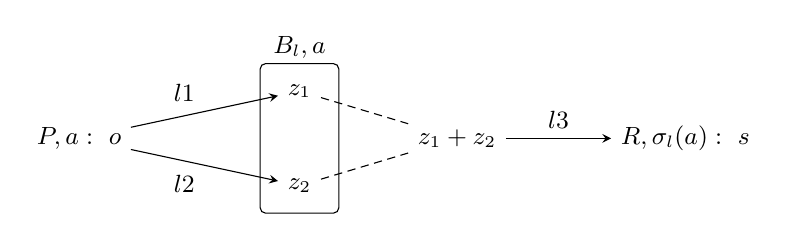
\begin{tikzpicture}[>=stealth, every node/.style={font=\small}]
 \node (source) at (0,0) {\(P,a:\ o\)};
 \node (one) at (2.8,.6) {\(z_1\)};
 \node (two) at (2.8,-.6) {\(z_2\)};
 \node at (2.8,1.15) {\(B_l,a\)};
 \draw[rounded corners=2pt] (2.3,-.95) rectangle (3.3,.95);
 \node (sum) at (4.8,0) {\(z_1+z_2\)};
 \node (target) at (7.7,0) {\(R,\sigma_l(a):\ s\)};
 \draw[->] (source) -- node[above left] {\(l1\)} (one);
 \draw[->] (source) -- node[below left] {\(l2\)} (two);
 \draw[densely dashed] (one) -- (sum);
 \draw[densely dashed] (two) -- (sum);
 \draw[->] (sum) -- node[above] {\(l3\)} (target);
\end{tikzpicture}
\caption{A buffered connection.  Solid arrows represent the three comparisons
in \eqref{eq:buffer}; dashed lines indicate addition of the two coordinates,
not further comparisons.  Image consistency compares sets of form values,
with their shifts.  It does not choose a common pointwise value for all
comparisons.}
\label{fig:buffer}
\end{figure}

Apply the layout and graph construction to exactly the seed comparisons and
the triples \eqref{eq:buffer}, and output
\begin{equation}
 (G(0),r),
 \label{eq:reduction-output}
\end{equation}
with \(r\) as in \eqref{eq:computation-parameters}.  All real-type dimensions
are one or two, all domains are nonempty products, and all address maps are
coordinate injections.  Thus the hypotheses of the graph construction hold.

\subsection{Acceptance: every equivalent mate is isomorphic}

\begin{proposition}
\label{prop:acceptance}
If \(M\) accepts \(w\), then every finite simple uncolored graph
\(H\equiv_r G(0)\) is isomorphic to \(G(0)\).
\end{proposition}

\begin{proof}
By Proposition~\ref{prop:mate}, write \(H\cong G(\beta)\) for some square
bits \(\beta\).  Transporting equivalence through this isomorphism, apply
Proposition~\ref{prop:image-consistency} to obtain nonempty sets
\(Q_{P,a}\) satisfying \eqref{eq:image-consistency}.  No restriction to the
special twists of Theorem~\ref{thm:special-twist} is made here: all wire sums
\(\Delta_e(a)\) may depend on the address.

First consider a buffered connection \(l\) at \(a\in D_l\).  If the source
image \(o(Q_{P,a})\) is a singleton, the first two comparisons force both
coordinate images of \(Q_{B_l,a}\) to be singletons, possibly translated by
different shifts.  As this set is nonempty, it contains exactly one vector.
Its sum image is therefore a singleton, and the third comparison makes
\(s(Q_{R,\sigma_l(a)})\) a singleton.  Thus a buffered connection propagates
singletonness from its source form to its destination form.  We do not need
these singletons to have value zero.

At each seed, comparison with the dummy's zero form gives a singleton scalar
image.  Induction in the acyclic circuit order now shows that every true gate
has a singleton output image.  For a true scalar, use its seed comparison or
one true incoming source.  For a true AND gate, each port receives a true
source, so both coordinate images become singletons and their sum is a
singleton as well.

By Proposition~\ref{prop:computation}, at least one test is true.  Its added
connection forces \(A\) to have a singleton image at that address.  Flipping
individual coordinates connects all addresses in \(\{0,1\}^r\), so the
broadcast connections propagate this property to every address of \(A\).
The connections from \(A\) to every gate coordinate then imply that all
primary sets are singletons.  Write
\[
 Q_{P,a}=\{h_P(a)\}
 \qquad(P\text{ primary},\ a\in\{0,1\}^r).
\]

To use Proposition~\ref{prop:global-offsets}, it remains to prove that these
functions have row-sum form and to supply the functions at the remaining real
types.  Fix a coordinate form \(s\) of a primary type \(P\), and take its
identity self-connection \(l\).  At each address, the first two comparisons
give buffer coordinates
\[
 z_1=s(h_P(a))+\Delta_{l1}(a),\qquad
 z_2=s(h_P(a))+\Delta_{l2}(a).
\]
Their sum cancels the two copies of \(s(h_P(a))\) over \(\F\).  The third
comparison, with destination the same coordinate at the same address, gives
\begin{equation}
 s(h_P(a))=\Delta_{l1}(a)+\Delta_{l2}(a)+\Delta_{l3}(a).
 \label{eq:self-connection-row-sum}
\end{equation}
Each term on the right has row-sum form on the full product.  Hence every
coordinate of every primary \(h_P\) has row-sum form, and therefore so does
the vector function itself.  Either self-connection copy suffices for \(A\).

For each private buffer \(B_l\), prescribe on \(D_l\) its coordinates
\[
 h_{B_l,j}(a)=o(h_P(a))+\Delta_{lj}(a),\qquad j=1,2.
\]
These are the unique coordinates of its image-consistency set on that domain.
They have row-sum form there.  Extend each adjacent-coordinate term arbitrarily
from its allowed pair of factors to \(\{0,1\}^2\); their sums define row-sum
functions on the full address product.  This extension changes no comparison,
because the buffer occurs only in its three schemas on \(D_l\).  Give the
dummy the zero function.

On each comparison domain, every scalar form appearing in a comparison now has
the singleton value prescribed by Equation~\eqref{eq:image-consistency}; the
dummy's zero form also has its required singleton image.  Thus these row-sum
functions satisfy all identities in
\eqref{eq:global-offsets}.  Proposition~\ref{prop:global-offsets} supplies
global offsets, and Proposition~\ref{prop:isomorphism} gives
\(G(\beta)\cong G(0)\).  Therefore \(H\cong G(0)\), as required.
\end{proof}

\subsection{Nonacceptance: an equivalent nonisomorphic mate}

\begin{proposition}
\label{prop:rejection}
If \(M\) does not accept \(w\), then there is a choice of square bits
\(\beta\) such that \(G(\beta)\equiv_r G(0)\) but
\(G(\beta)\not\cong G(0)\).
\end{proposition}

\begin{proof}
Choose comparison constants \(b_e\in\F\) as follows.  All are zero except
the constant of the third comparison of one of the two identity
self-connections at \(A\), which is one.  Form the special twist of
Theorem~\ref{thm:special-twist}: on each wire put \(b_e\) on its last link
and zero on its other links, and on a square in row \(i\) use that link
constant multiplied by \(\delta_i\), where \(\delta_r=1\) and all other
\(\delta_i=0\).  Then \(\Delta_e(a)=b_e\) on every comparison domain.

We first rule out an isomorphism.  In a hypothetical solution of
\eqref{eq:global-offsets}, the first two comparisons of either broadcast
self-connection would copy \(h_A(a)\) into both coordinates of that
connection's buffer.  Their sum would be zero.  The unshifted copy's third
comparison would force \(h_A(a)=0\), whereas the shifted copy's third
comparison would force \(h_A(a)=1\).  This contradiction holds at every
address.  Propositions~\ref{prop:global-offsets} and
\ref{prop:isomorphism} therefore show that \(G(\beta)\not\cong G(0)\).

To prove equivalence, it suffices by Theorem~\ref{thm:special-twist} to
construct nonempty image-consistency sets.  Evaluate truth only in the
original acyclic circuit.  At a scalar gate use \(\{0\}\) if it is true
and \(\F\) if it is false.  At an AND gate, use the product subset of
\(\F^2\) whose coordinate is fixed to zero if its corresponding port is
true and is free otherwise.  Its output sum image is \(\{0\}\) exactly
when both ports are true, and is \(\F\) otherwise.  Thus every gate output
has image \(\{0\}\) if true and \(\F\) if false.  Give both \(A\) and
the dummy the full set \(\F\) at every address.  The seed comparisons
hold, since a seed is true and the image of the zero form at the dummy is
\(\{0\}\).

Consider any unshifted directed connection \(l\).  A singleton source image
is necessarily \(\{0\}\), and its destination image is then also
\(\{0\}\).  For an original circuit edge this follows because a true
source makes the destination scalar or input port true.  For an identity
self-connection it is immediate.  All tests are false in the present case,
and all broadcast sources have full images, so those added connections
produce no further singleton-source case.  In the singleton-source case
choose
\[
 Q_{B_l,a}=\{(0,0)\}.
\]
Its two coordinate images and its sum image satisfy all three comparisons.

In every other case, including the shifted broadcast self-connection, the
source image is \(\F\).  Let
\(D'=s(Q_{R,\sigma_l(a)})\) be the nonempty destination image, and choose
\begin{equation}
 Q_{B_l,a}=\{(u,v)\in\F^2:u+v\in D'+b_{l3}\}.
 \label{eq:rejecting-buffer-set}
\end{equation}
Both coordinate projections of this set are \(\F\), and its sum image is
exactly \(D'+b_{l3}\).  Since \(b_{l1}=b_{l2}=0\) throughout, all three
comparisons again hold.  This includes a full source image and a singleton
destination image: the buffer may have two correlated coordinates without
either projection being a singleton.  That possibility is why image
consistency does not imply a global pointwise solution here.

These choices define each private buffer on its active domain.  Extend it by
arbitrary nonempty sets outside that domain, where it occurs in no comparison.
We have obtained nonempty sets at every real type and address satisfying
\eqref{eq:image-consistency} with shifts \(b_e\).  Theorem~\ref{thm:special-twist}
therefore gives \(G(\beta)\equiv_r G(0)\).
\end{proof}

\subsection{Polynomial size and the main theorem}

The circuit description uses \(O_M((r+1)^2+m)\) schemas and requests, and
the added directed connections use only \(O_M(r+1)\) schemas.  Buffering
adds a constant number of real types and comparison schemas per connection.
Since \(r\ge m\), there are \(O_M((r+1)^2)\) real types and comparisons.
Subdividing each comparison wire into \(4(r+1)+1\) links gives
\(O_M((r+1)^3)\) layout types and links.

For each row and type there are at most four horizontal label pairs, and for
each row and link at most four matched label pairs defining squares.  The
dimensions are at most two and the legal valuation classes have bounded size.
Consequently the number \(J\) of colors and the number \(N\) of base vertices
both satisfy
\[
 J,N=O_M((r+1)^4).
\]
The color-removing leaves add at most \(NJ(N+1)\) vertices, so the uncolored
graph has order \(O_M((r+1)^{12})\).  All its local data can be generated
from coordinate tables and adjacent pairs of coordinate labels.  Enumerating
the constant-dimensional valuations, the private leaf indices, and finally
every pair of output vertices constructs the full binary adjacency matrix in
polynomial time in \(r+m\).  There is no enumeration of full computation
addresses.  The graph is nonempty and simple, and the positive integer
\(r=2p(m)+4\) can be computed and written in binary in polynomial time.

\begin{proof}[Proof of Theorem~\ref{thm:main}]
Proposition~\ref{prop:upper} gives membership in \(\mathrm{EXPTIME}\).
For hardness, fix any language in \(\mathrm{EXPTIME}\) and its machine
\(M\) as above.  The construction \eqref{eq:reduction-output} is a
deterministic polynomial-time map from its input words to graph--parameter
pairs.  If \(M\) accepts, Proposition~\ref{prop:acceptance} says that
\(r\)-WL identifies \(G(0)\), so its dimension is at most \(r\).
If \(M\) does not accept, Proposition~\ref{prop:rejection} supplies an
equivalent nonisomorphic graph, so \(r\)-WL does not identify \(G(0)\).
By monotonicity of identification in the dimension, the dimension of
\(G(0)\) is then greater than \(r\).  Thus acceptance maps exactly to the
YES instances of the dimension problem.  Since the language was arbitrary,
the problem is \(\mathrm{EXPTIME}\)-hard under deterministic polynomial-time
many-one reductions, and hence \(\mathrm{EXPTIME}\)-complete.
\end{proof}

\begin{corollary}\label{cor:unary}
The identification problem of Theorem~\ref{thm:main} remains
EXPTIME-complete when the positive dimension is encoded in unary.
\end{corollary}
\begin{proof}
For membership, convert the unary dimension to binary and apply
Proposition~\ref{prop:upper}. For hardness, the reduction above outputs
\(r=2p(m)+4\), whose value is polynomial in the source input length
\(m\). Writing \(r\) in unary therefore preserves polynomial-time
constructibility and the same acceptance equivalence.
\end{proof}
